%%%%%%%%%%%%%%%%%%%%%%%%%%%%%%%%%%%%%%%%%
% Journal Article
% LaTeX Template
% Version 1.3 (9/9/13)
%
% This template has been downloaded from:
% http://www.LaTeXTemplates.com
%
% Original author:
% Frits Wenneker (http://www.howtotex.com)
%
% License:
% CC BY-NC-SA 3.0 (http://creativecommons.org/licenses/by-nc-sa/3.0/)
%
%%%%%%%%%%%%%%%%%%%%%%%%%%%%%%%%%%%%%%%%%

%----------------------------------------------------------------------------------------
%	PACKAGES AND OTHER DOCUMENT CONFIGURATIONS
%----------------------------------------------------------------------------------------

\documentclass{article}

\usepackage{mathtools} %tools for mathematical writing
\usepackage{caption}
\usepackage{subfig}
\usepackage{float}
\usepackage{color}
\usepackage{adjustbox}

\usepackage[sc]{mathpazo} % Use the Palatino font
\usepackage[T1]{fontenc} % Use 8-bit encoding that has 256 glyphs
\linespread{1.05} % Line spacing - Palatino needs more space between lines
\usepackage{microtype} % Slightly tweak font spacing for aesthetics

\usepackage[hmarginratio=1:1,top=32mm,columnsep=20pt]{geometry} % Document margins
%\usepackage{multicol} % Used for the two-column layout of the document
%\usepackage[hang, small,labelfont=bf,up,textfont=it,up]{caption} % Custom captions under/above floats in tables or figures
\usepackage{booktabs} % Horizontal rules in tables
%\usepackage{float} % Required for tables and figures in the multi-column environment - they need to be placed in specific locations with the [H] (e.g. \begin{table}[H])
\usepackage{hyperref} % For hyperlinks in the PDF

\usepackage{lettrine} % The lettrine is the first enlarged letter at the beginning of the text
\usepackage{paralist} % Used for the compactitem environment which makes bullet points with less space between them

\usepackage{abstract} % Allows abstract customization
\renewcommand{\abstractnamefont}{\normalfont\bfseries} % Set the "Abstract" text to bold
\renewcommand{\abstracttextfont}{\normalfont\small\itshape} % Set the abstract itself to small italic text

\usepackage{titlesec} % Allows customization of titles
%\renewcommand\thesection{\Roman{section}} % Roman numerals for the sections
%\renewcommand\thesubsection{\Roman{subsection}} % Roman numerals for subsections
\titleformat{\section}[block]{\large\scshape\centering}{\thesection.}{1em}{} % Change the look of the section titles
\titleformat{\subsection}[block]{\large}{\thesubsection.}{1em}{} % Change the look of the section titles

\usepackage{fancyhdr} % Headers and footers
\pagestyle{fancy} % All pages have headers and footers
\fancyhead{} % Blank out the default header
\fancyfoot{} % Blank out the default footer
%\fancyhead[C]{Running title $\bullet$ November 2012 $\bullet$ Vol. XXI, No. 1} % Custom header text
\fancyfoot[RO,LE]{\thepage} % Custom footer text

\usepackage{algorithm}% http://ctan.org/pkg/algorithms
\usepackage{algpseudocode}% http://ctan.org/pkg/algorithmicx

\usepackage[acronym]{glossaries} %Used for the acronyms

\usepackage{tikz}	%Used for the drawings
\usetikzlibrary{arrows, calc,decorations.pathmorphing,positioning,decorations.markings}

\DeclarePairedDelimiter\ceil{\lceil}{\rceil}
\DeclarePairedDelimiter\floor{\lfloor}{\rfloor}

%My definitions
%\renewcommand{\tablename}{Table}

\newtheorem{theorem}{Theorem}
\newtheorem{proposition}{Proposition}[section]
\newtheorem{corollary}{Corollary}[theorem]
\newtheorem{remark}{Remark}
\newenvironment{proof}{\begin{trivlist} \item[]\textbf{Proof}
\hspace{0cm} }{\hfill $\Box$ \end{trivlist}}
\newtheorem{mydef}{Definition}[section]
%\newcommand{\eqref}[1]{\mbox{(\ref{#1})}}
\newcommand{\Tr}{\mbox{Tr}}

%Set space between paragraphs
\setlength{\parskip}{2ex}

\usepackage{authblk}
%----------------------------------------------------------------------------------------
%	TITLE SECTION
%----------------------------------------------------------------------------------------

\title{Computational Power Analysis}
\author[1]{David Laredo\thanks{dlaredorazo@usmerced.edu}}

\date{}
%\renewcommand\Authands{ and }

% Generate the glossary
%\makeglossaries
%\renewcommand*{\acronymname}{Acronyms}

%----------------------------------------------------------------------------------------

%----------------------------------------------------------------------------------------
%	FIGURE CONFIGURATION
%----------------------------------------------------------------------------------------
\tikzset{
    shadedrec/.style={
        rectangle,
        draw=black,
        top color=gray, 
        bottom color=white, 
        shading angle={135},
        text width=3cm,
        inner sep=1em,
        rounded corners=1.2ex,
        very thick,
        text centered},
    snake arrow/.style={
        decorate,
        decoration={zigzag,amplitude=3mm,segment length=5mm,post length=0mm}},
    damper/.style={
        very thick,
        decoration={markings,  
        mark connection node=dmp,
        mark=at position 0.5 with 
        {
            \node (dmp) [very thick,transform shape,text width=.3cm,rotate=-90,minimum height=3pt,draw=none, fill=black,outer xsep=2pt, outer ysep=1pt] {};
            \draw [very thick] ($(dmp.north east)+(-.6pt,0)$) -- ($(dmp.south east)+(-.6pt,0)$) -- ($(dmp.south west)+(-.6pt,0)$) -- ($(dmp.north west)+(-.6pt,0)$);
            \draw [very thick,rotate=-90] ($(dmp.north)+(0,-5pt)$) -- ($(dmp.north)+(0,5pt)$);
        }
    }, decorate}
}
%----------------------------------------------------------------------------------------

\begin{document}

\maketitle % Insert title

\thispagestyle{fancy} % All pages have headers and footers

%Term definitions
\newacronym{moo}{MOO}{Multi-objective Optimization}
\newacronym{mop}{MOP}{Multi-objective Optimization Problem}
\newacronym{mmop}{MMOP}{Mixed-Integer Multi-objective Optimization Problem}
\newacronym{eds}{EDS}{Enhanced Directed Search}
\newacronym{dzz}{DZZ}{Direct Zig Zag}
\newacronym{nsga2}{NSGA-II}{Non-Sorted Genetic Algorithm II}
\newacronym{sop}{SOP}{Single-objective Optimization Problem}
\newacronym{pc}{PC}{Predictor-Corrector}
\newacronym{moea}{MOEA}{Multi-objective Optimization Evolutionary Algorithm}
\newacronym{ea}{EA}{Evolutionary Algorithm}
\newacronym{ds}{DS}{Directed Search}
\newacronym{kkt}{KKT}{Karush-Kuhn-Tucker}
\newacronym{bop}{BOP}{Bi-objective Optimization Problem}
\newacronym{gd}{GD}{Generational Distance}
\newacronym{igd}{IGD}{Inverted Generational Distance}
\newacronym{gsa}{GSA}{Gradient Subspace Approximation}
\newacronym{ift}{IFT}{Implicit Function Theorem}
\newacronym{fps}{FPS}{First Pareto Solution}
\newacronym{moead}{MOEA-D}{Multi-objective Optimization Evolutionary Algorithm based on Decomposition}
\newacronym{pf}{PF}{Pareto Front}
\newacronym{nbi}{NBI}{Normal Boundary Intersection}
\newacronym{pso}{PSO}{Particle Swarm Optimization} %Insert acronym list

%Used to not expand the first acronym
\glsunsetall

%----------------------------------------------------------------------------------------
%	ABSTRACT
%----------------------------------------------------------------------------------------

\begin{abstract}

\noindent 

The following report presents an analysis of the asympotic complexity of the proposed algorithms to be used for the development of the inteligent HVAC system as well as a brief analysis on the computational power of the computer we have destined for our experiments. Based on these two analysis we will draw our conclusions on whether the available computational power is enough for the development of our project.

\end{abstract}

%----------------------------------------------------------------------------------------
%	ARTICLE CONTENTS
%----------------------------------------------------------------------------------------

%Asymptotic Complexities of the Proposed Algorithms
%Computational Power of the available equipment
\section{Computational Complexities of the Algorithms}

\lettrine[nindent=0em,lines=3]{I}n this chapter we will briefly discuss each one of the algorithms intended to be used in the development of the Intelligent HVAC System. Along with the description of such algorithms we will present a very brief analysis on their computational complexity.

\subsection{Artificial Neural Network}

Artificial Neural Networks (ANNs) are computing systems inspired by the biological networks that constitute the brain. Such systems learn (progressively improve performance) to do tasks by considering examples, generally without task-specific programming. 

An ANN is based on a collection of connected units called artificial neurons, (analogous to axons in a biological brain). Each connection (synapse) between neurons can transmit a signal to another neuron. The receiving (postsynaptic) neuron can process the signal(s) and then signal downstream neurons connected to it. Neurons may have state, generally represented by real numbers, typically between 0 and 1. Neurons and synapses may also have a weight that varies as learning proceeds, which can increase or decrease the strength of the signal that it sends downstream. Further, they may have a threshold such that only if the aggregate signal is below (or above) that level is the downstream signal sent. Typically, neurons are organized in layers. Different layers may perform different kinds of transformations on their inputs. Signals travel from the first (input), to the last (output) layer, possibly after traversing the layers multiple times. \cite{ann_wikipedia}

The multilayer perceptron is an artificial neural network structure and is a nonparametric estimator that can be used for classification and regression. It is a supervised learning algorithm that learns a function $f(\cdot): R^m \rightarrow R^o$ by training on a dataset, where $m$ is the number of dimensions for input and $o$ is the number of dimensions for output. Given a set of features $X = {x_1, x_2, ..., x_m}$ and a target $y$, it can learn a non-linear function approximator for either classification or regression. It is different from logistic regression, in that between the input and the output layer, there can be one or more non-linear layers, called hidden layers. Figure \ref{Fig:mlp_example} shows a one hidden layer MLP with scalar output. \cite{ann_scikit}

\begin{figure}[H]
\centering 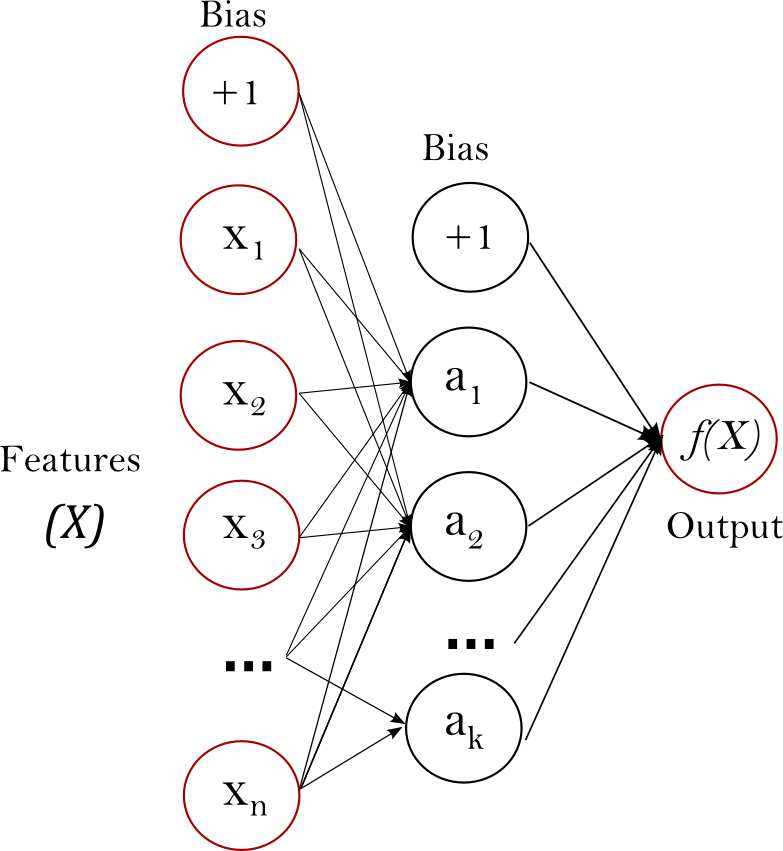
\includegraphics[width = 60mm, height = 60mm]{imgs/multilayerperceptron_network.png}
\caption{Multilayer perceptron}
\label{Fig:mlp_example}
\end{figure}

The leftmost layer, known as the input layer, consists of a set of neurons $\{x_i | x_1, x_2, ..., x_m\}$ representing the input features. Each neuron in the hidden layer transforms the values from the previous layer with a weighted linear summation $w_1x_1 + w_2x_2 + ... + w_mx_m$, followed by a non-linear activation function $g(\cdot):R \rightarrow R$ - like the hyperbolic tan function. The output layer receives the values from the last hidden layer and transforms them into output values.

The advantages of multilayer perceptrons are:
 \begin{itemize}
 \item Capability to learn non-linear models
 \item Capability to learn models in real-time (on-line learning)
 \end{itemize}
 
 The disadvantages of multilayer perceptron (MLP) include:
 \begin{itemize}
 \item MLP with hidden layers have non-convex cost function where there exists more than one local minimum. Therefore different random weight initializations can lead to different validation accuracy.
 \item MLP requires the tuning number of of hyperparameters such as the \textit{number of hidden neurons, layers and iterations}.
 \item MLP is sensitive to feature scaling
 \end{itemize}
 
 \subsubsection{Computational Complexity}
 
Suppose there are $n$ training samples, $m$ features, $k$ hidden layers, each containing $h$ neurons - for simplicity, and $o$ output neurons. The time complexity of the feedforward-backpropagation algorithm is 

\begin{equation}
O(n\cdot m \cdot h^k \cdot o)
\label{eq:ann_complexity1}
\end{equation}

Also for the sake of simplicity lets assume that $m>h>o$, hence the time complexity for feedforward-backpropgation algorithm is 

\begin{equation}
O(n\cdot m^{k+2})
\label{eq:ann_complexity2}
\end{equation}

Additional to the computation of the gradients using the backpropagation algorithm we need to consider the complexity (convergence ratio) of the algorithm used for solving the minimization problem inherent to the neural network, recall that at each iteration a minimization problem is solved. For the best case, this is superlinear (L-BFGS) and for the worst case it is linear (Stochastic Gradient Descent).

\subsection{Anomaly Detection}
\label{sec:anomaly_detection_alg}

Assume we have a sample $\mathbb{M}$ drawn from the same distribution. An outlier, novelty, or anomaly is an instance that is very much different from other instances in the sample. An outlier may indicate an abnormal behavior of the system; for example, in a dataset of credit card transactions, it may indicate fraud; in an image, outliers may indicate anomalies, for example, tumors. \cite{intro_to_machine_learning}

Outlier detection is not generally cast as a supervised, two-class clas- sification problem of seperating typical instances and outliers, because generally there are very few instances that can be labeled as outliers and they do not fit a consistent pattern that can be easily captured by a two- class classifier. Instead, it is the typical instances that are modeled; this is sometimes called one-class classification. Once we model the typical instances, any instance that does not fit the model (and this may occur in many different ways) is an anomaly.

Outlier detection basically implies spotting what does not normally happen; that is, it is density estimation followed by checking for in- stances with too small probability under the estimated density. As usual, the fitted model can be parametric, semiparametric, or nonparametric. In the parametric case, for example, we can fit a Gaussian to the whole data and any instance having a low probability, or equally, with high Mahalanobis distance to the mean, is a candidate for being an outlier. \cite{anomaly_scikit}

Figure \ref{Fig:noveltyDetection_example} shows how novelty detection can separate data into regular observations and abnormal observations.

\begin{figure}[H]
\centering 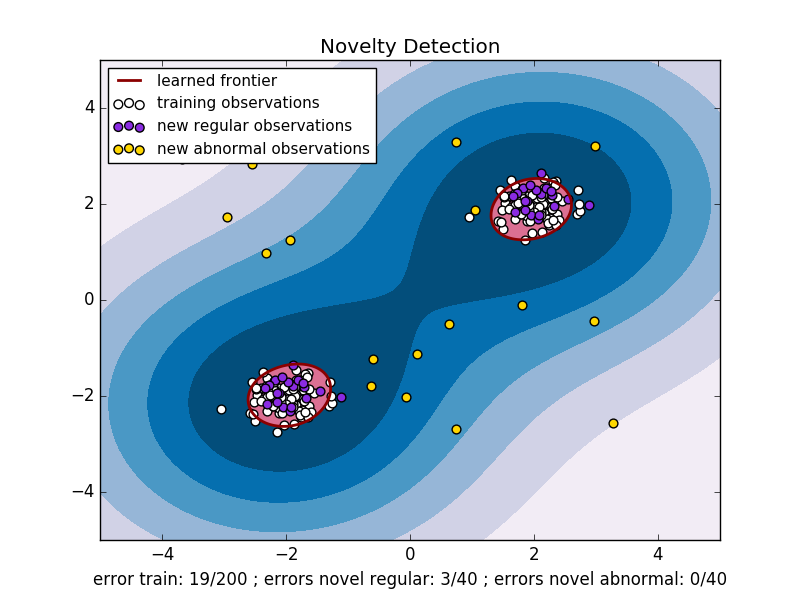
\includegraphics[width = 90mm, height = 40mm]{imgs/noveltyDetection.png}
\caption{Novelty detection}
\label{Fig:noveltyDetection_example}
\end{figure}

One common way of performing outlier detection is to assume that the regular data come from a known distribution (e.g. data are Gaussian distributed). From this assumption, we generally try to define the “shape” of the data, and can define outlying observations as observations which stand far enough from the fit shape. The process for defining the "shape" of the data is as follows and assumes that all of the samples come from a known distribution, say Gaussian for the purposes of this explanation.

Assume a training set $T = \{x^{(1)}, \cdots, x^(m) \}$ where $x \in \mathbb{R}^n$. Suppose that each feature $x_i from x$ is distributed according to some Gaussian distribution $x_i \sim \mathcal{N}(\mu_i, \sigma_i^2)$. Hence $p(x) = \prod_{j = 1}^n p(x_j; \mu_j, \sigma_j^2)$. The task is now to find the corresponding means $\mu_i$ for $i = 1,\cdots,n$ and standard deviations $\sigma_i^2$ for  $i = 1,\cdots,n$ of the $n$ different distributions. This can be easily done for the Gaussian distribution as follows

\begin{equation}
\mu_j = \frac{1}{m} \sum_{i=1}^{m} x_j^{(i)}
\label{eq:mean_eq_gaussian}
\end{equation}

and

\begin{equation}
\sigma_j^2 = \frac{1}{m} \sum_{i=1}^{m} (x_j^{(i)} - \mu_j)^2
\label{eq:std_eq_gaussian}
\end{equation}

We can now describe the simplest anomaly detection algorithm

\begin{enumerate}
\item Choose features $x_i$ that might be indicative/sensitive of/to anomalies.
\item Fit parameters $\mu_1, \cdots, \mu_n$ and $\sigma_1^2,\cdots, \sigma_n^2$ using equations \eqref{eq:mean_eq_gaussian} and \eqref{eq:std_eq_gaussian} respectively.
\item Given a new example $x$, compute $p(x) = \prod_{j = 1}^n p(x_j; \mu_j, \sigma_j^2)$ 
\item Tag the new sample $x$ as an anomaly if $p(x) < \epsilon$, where $epsilon$ is a hyperparameter defined by the user.
\end{enumerate}

 \subsubsection{Computational Complexity}

Usually the complexity of this algorithm is negligible compared to the complexity of the feedforward-backpropagation algorithm. As can be seen from the Algorithm in Section \ref{sec:anomaly_detection_alg} the asymptotic complexity of such algorithm is $O(n)$ where $n$ is the number of choosen features.
\section{Computational Power of the Equipment}

\lettrine[nindent=0em,lines=3]{I}n this chapter we present an analysis on the features of the available equipment for our experiments and final implementation of the system. We will make emphasis on the number of operations per second (FLOPS) that our equipment can handle.

Floating Point Operations per Second (FLOPS) is a measure of computer performance, useful in fields of scientific computations that require floating-point calculations. For such cases it is a more accurate measure than measuring instructions per second \cite{flops_wikipedia}. The FLOPS value can be used to determine the power for both the CPU and GPU.

The amount of Giga FLOPS (GFLOPS) for each node/computer can be calculated by using the following equation \cite{peak_theoretical_performance}.

\begin{equation}
GFLOPS = \textit{CPU speed in GHz} \times \textit{number of CPU cores} \times \textit{CPU instruction per cycle} \times \textit{number of CPUs per node} 
\label{flops_eq_cpu}
\end{equation}

For the case of Graphics Processing Units (GPUs), the amount of flops the GPU can support can be computed by \cite{gpu_flops}

\begin{equation}
FLOPS = 2 \times \textit{number of parallel GPU processing cores} \times \textit{peak clock speed in MHz}
\label{flops_eq_gpu}
\end{equation}

The computer used for our experiments has an Intel Core i7-7700K Processor; with a CPU speed of 4.2 GHz average and 4.5 GHz overclocked, 4 cores \cite{cpu_tech_specs}, and 16 IPC \cite{determine_number_flops_cpu}.  Using these values and eq. \eqref{flops_eq_cpu}, the FLOPS range for the CPU is: 268.8 GFLOPS to 288 GFLOPS.
    
The computer used for our experiments also comes with a dedicated GPU. The GPU used in our system is a NVDIA GeForce GTX 1080Ti with 11GB GDDR5X; with a boost clock of 1582 MHz and 3584 NVIDIA CUDA Cores \cite{gpu_tech_specs}. Using the given values and eq. \eqref{flops_eq_gpu} the FLOPS value for the GPU is 11339.776 GFLOPS which is approximately 11,300 GFLOPS.

By combining the FLOPs value for both the CPU and GPU, the total FLOPs range of the server is 11608.576 GFLOPS to 11627.776 GFLOPS. This can be converted to FLOPS/month by multiplying the given range by $2592000$, using the assumption that a month is 30 days. This gives a final FLOPS/month of $3.00894 \times 10^{19}$ FLOPS/month to $3.01392 \times 10^{19}$ FLOPS/month.

\section{Our problem}

Part of our problem is the detection and classification of faults in the HVAC system of the SE2 building in the Merced campus of the University of California. Such system has an approximate of 2000 sensor and we take samples each 5 minutes. It is our intention to use data from the past 2 years to train our model, this gives us a size for the training set of $n = 210240$ training samples. Thus, lets assume that our ANN will have the following topology: $m = 2000$ for the 2000 input features (this is just a rough estimate since we will apply dimensionality reduction and feature extraction techniques to reduce this number as much as we can), $k = 4$ layers for an ANN of 1 input layer, 2 hidden layers and 1 output layer. In this case we assume that the number of output layers (fault classes) $o$ is much smaller than the number of input layers, we expect a number on the order of $100$ different types of faults, as for the number of neurons on each hidden layer we will set it arbitrary to $2000$ (the number of input neurons) as it has been shown that the number of hidden layers for other classification/regression problems is usually smaller than the number of input layers, thus, setting the number of hidden layers equal to the number of input layers will help us set a boundary on the number of computations.

Using the above information and eq. \eqref{eq:ann_complexity1} the asymptotic complexity of our ANN will be $O(210240 * 2000 * 2000^2 * 100) = O(1.6819 \times 10^{17})$ FLOPS, this neglecting the computational time spent on the minimization problem inherent to the computation of the weights for the ANN.

\section{Conclusions}

Based on the estimate of FLOPS our equipment can handle which within the order of $3 \times 10^{19}$ FLOPS/month and the complexity for the training of our modeled ANN we estimate our which is of the order of $O(1.6819 \times 10^{17}$ FLOPS we conclude our system can do the training for our model in approximately one month of computations, provided that we take the most of our equipment, such as the pipe-lining and parallel computing.

%------------------------------------------------


%----------------------------------------------------------------------------------------
%	REFERENCE LIST
%----------------------------------------------------------------------------------------

\addcontentsline{toc}{section}{References}
\bibliographystyle{unsrt}
\bibliography{reference_computationalpower_analysis}

%----------------------------------------------------------------------------------------

\end{document}
